% Options for packages loaded elsewhere
\PassOptionsToPackage{unicode}{hyperref}
\PassOptionsToPackage{hyphens}{url}
\PassOptionsToPackage{dvipsnames,svgnames,x11names}{xcolor}
\documentclass[
  11pt,
  letterpaper,
]{article}
\usepackage{xcolor}
\usepackage[margin=1in]{geometry}
\usepackage{amsmath,amssymb}
\setcounter{secnumdepth}{5}
\usepackage{iftex}
\ifPDFTeX
  \usepackage[T1]{fontenc}
  \usepackage[utf8]{inputenc}
  \usepackage{textcomp} % provide euro and other symbols
\else % if luatex or xetex
  \usepackage{unicode-math} % this also loads fontspec
  \defaultfontfeatures{Scale=MatchLowercase}
  \defaultfontfeatures[\rmfamily]{Ligatures=TeX,Scale=1}
\fi
\usepackage{lmodern}
\ifPDFTeX\else
  % xetex/luatex font selection
\fi
% Use upquote if available, for straight quotes in verbatim environments
\IfFileExists{upquote.sty}{\usepackage{upquote}}{}
\IfFileExists{microtype.sty}{% use microtype if available
  \usepackage[]{microtype}
  \UseMicrotypeSet[protrusion]{basicmath} % disable protrusion for tt fonts
}{}
\usepackage{setspace}
\makeatletter
\@ifundefined{KOMAClassName}{% if non-KOMA class
  \IfFileExists{parskip.sty}{%
    \usepackage{parskip}
  }{% else
    \setlength{\parindent}{0pt}
    \setlength{\parskip}{6pt plus 2pt minus 1pt}}
}{% if KOMA class
  \KOMAoptions{parskip=half}}
\makeatother
\usepackage{longtable,booktabs,array}
\newcounter{none} % for unnumbered tables
\usepackage{calc} % for calculating minipage widths
% Correct order of tables after \paragraph or \subparagraph
\usepackage{etoolbox}
\makeatletter
\patchcmd\longtable{\par}{\if@noskipsec\mbox{}\fi\par}{}{}
\makeatother
% Allow footnotes in longtable head/foot
\IfFileExists{footnotehyper.sty}{\usepackage{footnotehyper}}{\usepackage{footnote}}
\makesavenoteenv{longtable}
\usepackage{graphicx}
\makeatletter
\newsavebox\pandoc@box
\newcommand*\pandocbounded[1]{% scales image to fit in text height/width
  \sbox\pandoc@box{#1}%
  \Gscale@div\@tempa{\textheight}{\dimexpr\ht\pandoc@box+\dp\pandoc@box\relax}%
  \Gscale@div\@tempb{\linewidth}{\wd\pandoc@box}%
  \ifdim\@tempb\p@<\@tempa\p@\let\@tempa\@tempb\fi% select the smaller of both
  \ifdim\@tempa\p@<\p@\scalebox{\@tempa}{\usebox\pandoc@box}%
  \else\usebox{\pandoc@box}%
  \fi%
}
% Set default figure placement to htbp
\def\fps@figure{htbp}
\makeatother
\setlength{\emergencystretch}{3em} % prevent overfull lines
\providecommand{\tightlist}{%
  \setlength{\itemsep}{0pt}\setlength{\parskip}{0pt}}
% Layout additions for manuscript.tex and supplement.tex (pandoc inlines this file into each preamble).
\usepackage{url}                 % \path for file names, commits and hashes (breakable; see code_path.lua)
\usepackage{caption}
\captionsetup{font=small,labelformat=empty,justification=justified,singlelinecheck=false,list=no,skip=6pt}
\usepackage[section]{placeins}   % figures do not float past the end of their section
\usepackage{etoolbox}
\AtBeginEnvironment{longtable}{\small}
\setlength{\LTpre}{8pt}
\setlength{\LTpost}{8pt}
\raggedbottom
\setlength{\parskip}{3pt plus 1pt}
\makeatletter
\renewcommand{\@seccntformat}[1]{\csname the#1\endcsname\quad}
\def\fps@figure{!htbp}
\renewcommand{\topfraction}{0.9}
\renewcommand{\bottomfraction}{0.8}
\renewcommand{\textfraction}{0.07}
\renewcommand{\floatpagefraction}{0.8}
\makeatother
\ifPDFTeX
  % pdfLaTeX (for example on arXiv): every non-ASCII character of manuscript.tex and supplement.tex, which XeTeX takes
  % from the font. build.sh lists the non-ASCII characters of both files and stops if one is not declared here.
  \DeclareUnicodeCharacter{2212}{\ensuremath{-}}        % minus sign
  \DeclareUnicodeCharacter{00B1}{\ensuremath{\pm}}      % plus-minus sign
  \DeclareUnicodeCharacter{2265}{\ensuremath{\geq}}     % greater-than or equal to
  \DeclareUnicodeCharacter{2264}{\ensuremath{\leq}}     % less-than or equal to
  \DeclareUnicodeCharacter{00D7}{\ensuremath{\times}}   % multiplication sign
  \DeclareUnicodeCharacter{00B5}{\ensuremath{\mu}}      % micro sign
  \DeclareUnicodeCharacter{00FC}{\"{u}}                 % u with diaeresis (a reference author's name)
  \DeclareUnicodeCharacter{00E9}{\'{e}}                 % e with acute (a reference author's name)
  \DeclareUnicodeCharacter{00E1}{\'{a}}                 % a with acute (a reference author's name)
  \DeclareUnicodeCharacter{2081}{\ensuremath{_1}}
  \DeclareUnicodeCharacter{2082}{\ensuremath{_2}}
\fi
% The author line is long: set it in a centred paragraph that can wrap, not in the default unbreakable tabular.
\usepackage{titling}
\pretitle{\begin{center}\LARGE\bfseries}
\posttitle{\par\end{center}\vskip 0.4em}
\preauthor{\begin{center}\large\begin{minipage}{0.92\textwidth}\centering}
\postauthor{\end{minipage}\par\end{center}}
\predate{\begin{center}\normalsize}
\postdate{\par\end{center}}
% Table captions sit at the top of their longtable (table_captions.lua) and span the text width.
\setlength{\LTcapwidth}{\textwidth}
\usepackage{bookmark}
\IfFileExists{xurl.sty}{\usepackage{xurl}}{} % add URL line breaks if available
\urlstyle{same}
% fallback for those not using the hyperref driver hyperxmp:
\makeatletter
\@ifundefined{xmpquote}{\newcommand{\xmpquote}[1]{#1}}{}
\makeatother
\hypersetup{
  pdftitle={Sex-chromosome expression and annotated donor sex in drug-perturbation cell lines},
  pdfauthor={Mateenah Jahan and Marouen Ben Guebila},
  colorlinks=true,
  linkcolor={Maroon},
  filecolor={Maroon},
  citecolor={Blue},
  urlcolor={Blue},
  pdfcreator={LaTeX via pandoc}}

\title{Sex-chromosome expression and annotated donor sex in
drug-perturbation cell lines}
\author{Mateenah Jahan and Marouen Ben Guebila}
\date{}

\begin{document}
\maketitle

\setstretch{1.12}
\section*{Abstract}\label{abstract}
\addcontentsline{toc}{section}{Abstract}

Recorded donor sex may differ from sex-chromosome expression in cultured
cells. We scored 8 Y-chromosome genes and XIST in vehicle-treated
Tahoe-100M cells and classified each line as Y only, XIST only, both or
neither. Of 49 lines with a donor-sex label, 27 lacked the expression
pattern usually associated with it. Both scores were low in 14 of 33
male-labelled lines, and XIST was low in 12 of 16 female-labelled lines.
Label-independent patterns agreed with bulk RNA-seq of other cultures
for 47 of 49 lines. We assembled expression-state records for 1,123
lines across three perturbation atlases and public bulk RNA-seq.

We also applied an internally specified analysis plan to LINCS2020 L1000
responses from 41 lines in 11 lineages and 114 compounds. The
panel-level tests detected no association with Y expression or XIST. The
pooled Y estimate remained compatible with a difference whose magnitude
exceeded the 20\% margin, the XIST vehicle control raised a calibration
concern, and post hoc simulations showed low sensitivity. The
drug-response analysis is inconclusive. Measured expression and recorded
donor sex describe different properties of a cell line and should be
reported separately.

\section{Introduction}\label{introduction}

Drug-perturbation atlases record how cell lines respond to many
compounds. L1000 measures landmark genes and infers others (Subramanian
et al.~2017), while sci-Plex (Srivatsan et al.~2020) and Tahoe-100M
(Zhang et al.~2026) measure transcripts in single cells. These data are
used to train models of perturbation response (Adduri et al.~2025;
Gandhi et al.~2025, preprint) and to evaluate generalization to new cell
lines (Adduri et al.~2026).

Recorded donor sex enters these analyses as metadata and as a grouping
variable. The PIE model's source data include a field for sex (Verma et
al.~2026a, preprint; Verma et al.~2026b; Table S2). Cell-line studies
have compared drug sensitivity and gene dependency by sex (Saha et
al.~2024; Zeltser et al.~2025, preprint).

Cellosaurus records donor sex (Bairoch 2018). During cancer evolution
and culture, cells can lose Y-chromosome material or its expression (Qi
et al.~2023; Chen et al.~2025; Nguyen et al.~2026; Gertych et al.~2026).
Cancer cells can also lose or destabilize the inactive X chromosome
(Sirchia et al.~2005; Chaligné et al.~2015). Previous studies have
documented these discrepancies and examined associations between
measured chromosome expression and gene essentiality (Shah, McCormack
and Bradbury 2014; Flynn, Chang and Altman 2021; Shohat, Vol and Shifman
2022; Plaisier et al.~2025, preprint).

We classify Y-gene and XIST expression in vehicle cells from Tahoe-100M,
EmeraldBay, Tahoe Therapeutics' second atlas of 52 cell lines (Table S2;
\href{https://huggingface.co/datasets/tahoebio/EmeraldBay}{Tahoe
Therapeutics dataset}), and sci-Plex. We compare measured patterns with
donor labels, bulk RNA-seq from other cultures and STR Amelogenin
typing. A pilot informed the classification rules before the full
Tahoe-100M analysis. We then examine whether the patterns are associated
with LINCS2020 transcriptional drug response within lineage, using
expression calls from external RNA-seq. Earlier exploratory analyses of
these data are described in Note S19. Throughout, donor sex refers to
the recorded attribute, and marker patterns refer to measured expression
(Heidari et al.~2016; Boulicault et al.~2025).

\begin{figure}
\centering
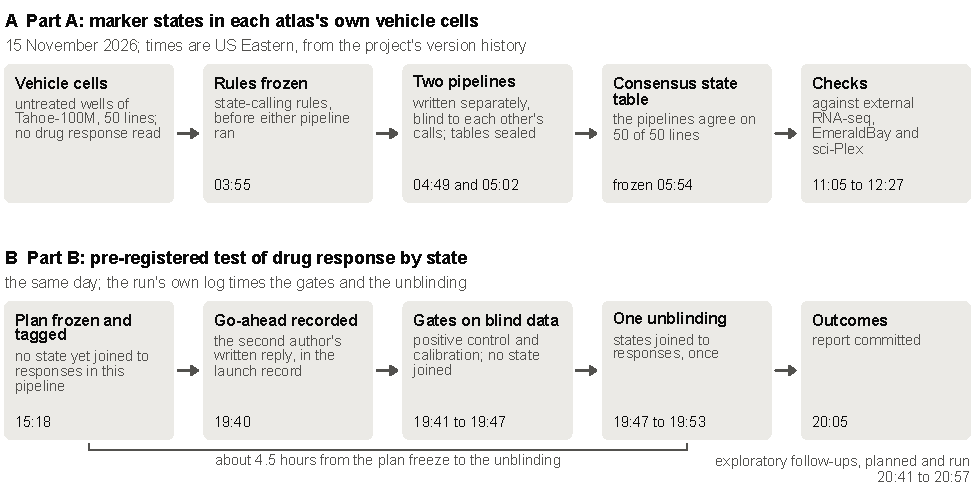
\includegraphics[width=1\linewidth,height=\textheight,keepaspectratio,alt={Figure 1. Study design and data sources. (A) Vehicle cells in the three atlases provide the Y-gene and XIST scores. Part A compares expression patterns with recorded donor sex and bulk RNA-seq from other cultures. STR Amelogenin typing supplies a separate check on the Y call. (B) Part B joins marker calls from external bulk RNA-seq to LINCS2020 drug responses. Within each lineage, the model compares Y-only and XIST-only lines with lines expressing neither marker and accounts for TP53 status. The analysis estimates panel-level, per-compound and pooled response-size differences.}]{figures/fig1_design.pdf}
\caption{\textbf{Figure 1. Study design and data sources.} (\textbf{A})
Vehicle cells in the three atlases provide the Y-gene and XIST scores.
Part A compares expression patterns with recorded donor sex and bulk
RNA-seq from other cultures. STR Amelogenin typing supplies a separate
check on the Y call. (\textbf{B}) Part B joins marker calls from
external bulk RNA-seq to LINCS2020 drug responses. Within each lineage,
the model compares Y-only and XIST-only lines with lines expressing
neither marker and accounts for TP53 status. The analysis estimates
panel-level, per-compound and pooled response-size differences.}
\end{figure}

\section{Results}\label{results}

\subsection{Part A: measured states in drug-atlas cell
lines}\label{part-a-measured-states-in-drug-atlas-cell-lines}

\subsubsection{The label audit}\label{the-label-audit}

In the 2,205,786 vehicle (DMSO) cells of the 50 Tahoe-100M lines, grown
in the same pooled culture as the treated cells, we scored XIST and a Y
score (the mean of 8 Y-chromosome genes) and set each cut-off at the
density minimum between the score's two modes (Methods).

Without reference to any label, 18 lines had a Y score at or above its
cut-off and XIST below its own (``Y only''), 6 had XIST without Y
(``XIST only''), 26 had neither marker high, and 0 had both (Figure 2A;
Table 1).

A male label, the donor sex that Cellosaurus records (Bairoch 2018),
usually goes with ``Y only'' and a female label with ``XIST only''. Of
the 49 labelled lines, 27 did not show their label's usual pattern: 14
of 33 male-labelled lines had neither marker high, although 3 of them
still had one Y-arm score above its cut-off; 12 of 16 female-labelled
lines had XIST below its cut-off; and A498, labelled male, expressed
XIST without Y. The count was unchanged with line-level cut-offs or the
PIE metadata label (Note S10). Expression surveys of cancer cell lines
found such mismatches before (Shohat, Vol and Shifman 2022; Plaisier et
al.~2025, preprint); here they are measured in the cultures that the
atlas treated.

\begin{longtable}[]{@{}llllll@{}}
\caption{\textbf{Table 1. Measured marker pattern of the Tahoe-100M
lines by Cellosaurus label.} Each cell gives the number of lines with
that label and pattern.}\tabularnewline
\toprule\noalign{}
Label & Lines & Y only & XIST only & neither & both \\
\midrule\noalign{}
\endfirsthead
\toprule\noalign{}
Label & Lines & Y only & XIST only & neither & both \\
\midrule\noalign{}
\endhead
\bottomrule\noalign{}
\endlastfoot
Male & 33 & 18 & 1 (A498) & 14 & 0 \\
Female & 16 & 0 & 4 & 12 & 0 \\
No label (RKO) & 1 & 0 & 1 & 0 & 0 \\
All & 50 & 18 & 6 & 26 & 0 \\
\end{longtable}

\begin{figure}
\centering
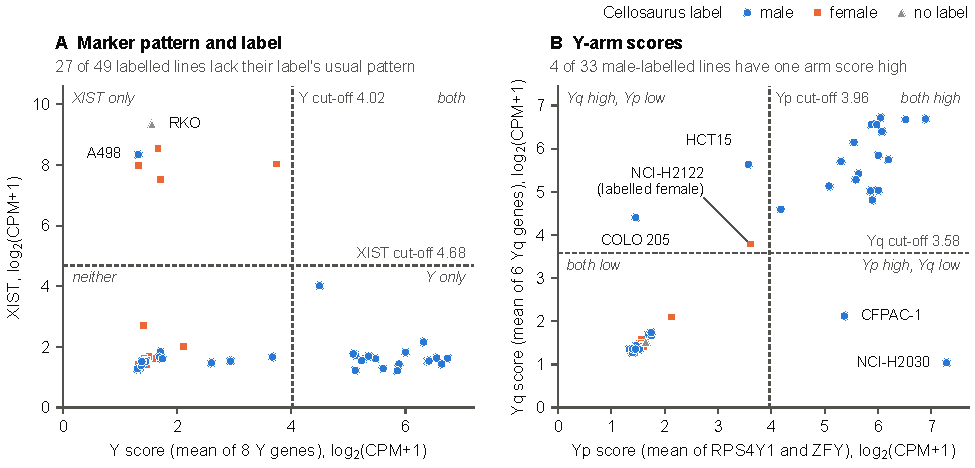
\includegraphics[width=1\linewidth,height=\textheight,keepaspectratio,alt={Figure 2. Annotated label against measured marker pattern in Tahoe-100M vehicle cells. One point per line (50 lines); marks give the Cellosaurus label. (A) XIST against the Y score, the mean of 8 Y genes, both in log2 counts per million plus one. Dashed lines mark the cut-offs (Y score 4.02, XIST 4.68), and the quadrants name the label-independent patterns; 27 of 49 labelled lines lack their label's usual pattern. (B) Yq score (mean of the six Yq genes) against Yp score (mean of RPS4Y1 and ZFY), with cut-offs 3.58 and 3.96. Quadrant names say which score is at or above its cut-off; they are thresholds, not chromosome states. Named lines have exactly one arm score high. NCI-H2122 is labelled female and its STR profile lacks AMELY. Its Yq signal may come from other lines' cells or RNA (Note S9).}]{figures/fig2_label_vs_pattern.pdf}
\caption{\textbf{Figure 2. Annotated label against measured marker
pattern in Tahoe-100M vehicle cells.} One point per line (50 lines);
marks give the Cellosaurus label. (\textbf{A}) XIST against the Y score,
the mean of 8 Y genes, both in log2 counts per million plus one. Dashed
lines mark the cut-offs (Y score 4.02, XIST 4.68), and the quadrants
name the label-independent patterns; 27 of 49 labelled lines lack their
label's usual pattern. (\textbf{B}) Yq score (mean of the six Yq genes)
against Yp score (mean of RPS4Y1 and ZFY), with cut-offs 3.58 and 3.96.
Quadrant names say which score is at or above its cut-off; they are
thresholds, not chromosome states. Named lines have exactly one arm
score high. NCI-H2122 is labelled female and its STR profile lacks
AMELY. Its Yq signal may come from other lines' cells or RNA (Note S9).}
\end{figure}

\subsubsection{Agreement across cultures and
assays}\label{agreement-across-cultures-and-assays}

The label-independent expression patterns agreed with external bulk
RNA-seq of other cultures for 47 of 49 lines (Figure 3A; Table 2). The
two different patterns were COLO 205, near the Y cut-off, and the
low-confidence NCI-H596, called from 345 cells (Note S9). State names agreed for 46 of 49 lines. Both cultures of A498
expressed XIST alone. Tahoe calls this pattern discordant in a male-labelled
line. The bulk RNA-seq rule calls the same pattern XX-like regardless of donor label.

For EmeraldBay, which cultured 47 shared lines separately, 40 of the 41
patterns called with high or medium confidence in both sources agreed
(Figure 3B). A-427 was the one different pattern among these confident
calls (Note S9). In sci-Plex, 5 of 6 line-by-experiment patterns matched
external RNA-seq. A549 in sciPlex3 also had XIST above the cut-off,
consistent with RNA or cells from other co-processed lines (Figure 3C;
Note S9).

In a post hoc check, the Tahoe-100M Y call agreed with AMELY status in
Cellosaurus STR profiles for 48 of 50 lines (Figure 3D; Note S14). This
count includes lines for which a Y marker is not expected. Among the 14
male-labelled lines with neither marker, 13 lacked AMELY in their STR
profile, consistent with loss of the measured locus in those stocks.
AMELY can be deleted independently of other Y loci (Steinlechner et
al.~2002; Thangaraj, Reddy and Singh 2002), and the STR profiles came
from other stocks. They cannot establish the structure of the Y
chromosome in the assayed cultures or resolve XIST status. Cancer cells
can express XIST from an active X chromosome (Sirchia et al.~2009).

\begin{longtable}[]{@{}
  >{\raggedright\arraybackslash}p{(\linewidth - 2\tabcolsep) * \real{0.5000}}
  >{\raggedright\arraybackslash}p{(\linewidth - 2\tabcolsep) * \real{0.5000}}@{}}
\caption{\textbf{Table 2. Agreement and measurement checks for Part
A.}}\tabularnewline
\toprule\noalign{}
\begin{minipage}[b]{\linewidth}\raggedright
Comparison
\end{minipage} & \begin{minipage}[b]{\linewidth}\raggedright
Outcome
\end{minipage} \\
\midrule\noalign{}
\endfirsthead
\toprule\noalign{}
\begin{minipage}[b]{\linewidth}\raggedright
Comparison
\end{minipage} & \begin{minipage}[b]{\linewidth}\raggedright
Outcome
\end{minipage} \\
\midrule\noalign{}
\endhead
\bottomrule\noalign{}
\endlastfoot
Tahoe-100M versus external bulk RNA-seq & 47 of 49 label-independent
patterns matched \\
Tahoe-100M versus EmeraldBay & 40 of 41 patterns called with high or
medium confidence in both cultures matched \\
sci-Plex versus external RNA-seq & 5 of 6 line-by-experiment patterns
matched \\
Tahoe-100M Y call versus STR AMELY status (post hoc) & 48 of 50 lines
agreed \\
Tahoe-100M plate consistency (post hoc) & 685 of 700 line-by-plate calls
matched the line call \\
\end{longtable}

\begin{figure}
\centering
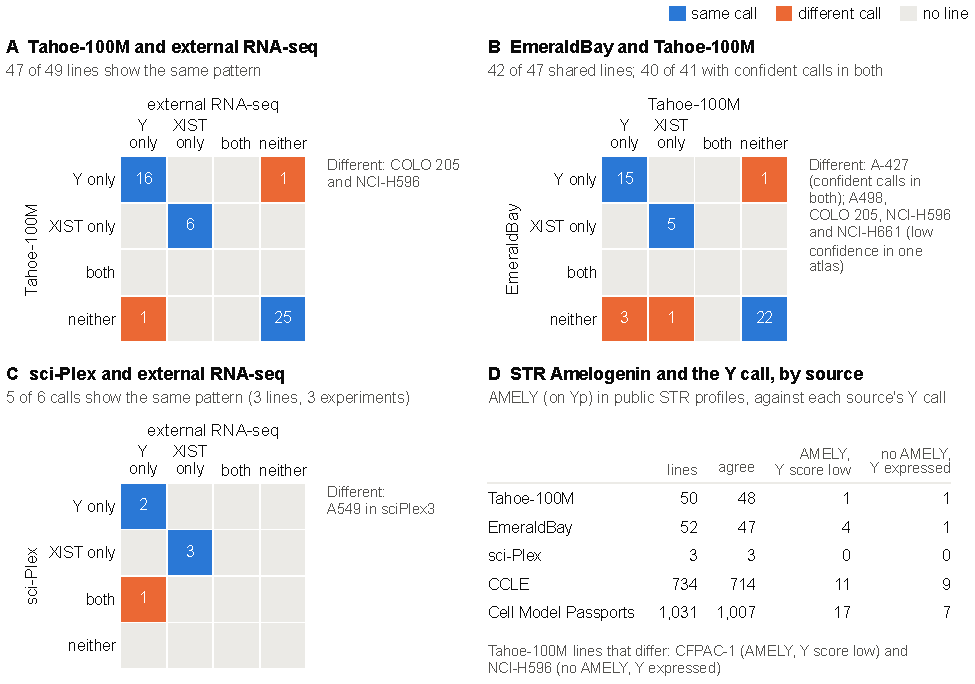
\includegraphics[width=1\linewidth,height=\textheight,keepaspectratio,alt={Figure 3. Agreement of the marker pattern across sources, and of the Y call with DNA. Each grid counts lines by the label-independent pattern that two sources give, each from its own scores and cut-offs; tiles on the diagonal hold lines called alike. (A) Tahoe-100M against external bulk RNA-seq of other cultures (47 of 49 patterns match). (B) EmeraldBay against Tahoe-100M (47 shared lines; 41 called with high or medium confidence in both). Patterns differed for A-427, COLO 205, A498, NCI-H596 and NCI-H661. Only A-427 had a high- or medium-confidence call in both atlases. (C) sci-Plex against external RNA-seq (6 line-by-experiment calls from three experiments). (D) Each source's Y call against the Amelogenin result of the line's STR profile in Cellosaurus, which tests for AMELY on the short arm of the Y; a line agrees if AMELY goes with a high Y score, or its absence with a low one. The post hoc STR comparison uses other stocks and tests a single locus.}]{figures/fig3_agreement.pdf}
\caption{\textbf{Figure 3. Agreement of the marker pattern across
sources, and of the Y call with DNA.} Each grid counts lines by the
label-independent pattern that two sources give, each from its own
scores and cut-offs; tiles on the diagonal hold lines called alike.
(\textbf{A}) Tahoe-100M against external bulk RNA-seq of other cultures
(47 of 49 patterns match). (\textbf{B}) EmeraldBay against Tahoe-100M
(47 shared lines; 41 called with high or medium confidence in both).
Patterns differed for A-427, COLO 205, A498, NCI-H596 and NCI-H661. Only
A-427 had a high- or medium-confidence call in both atlases.
(\textbf{C}) sci-Plex against external RNA-seq (6 line-by-experiment
calls from three experiments). (\textbf{D}) Each source's Y call against
the Amelogenin result of the line's STR profile in Cellosaurus, which
tests for AMELY on the short arm of the Y; a line agrees if AMELY goes
with a high Y score, or its absence with a low one. The post hoc STR
comparison uses other stocks and tests a single locus.}
\end{figure}

\subsubsection{Partial Y-marker
expression}\label{partial-y-marker-expression}

Among the 33 male-labelled lines, 17 had both Y-arm scores high, 12 both
low and 4 exactly one high (Figure 2B; Table S6). CFPAC-1 and NCI-H2030
had a high Yp score and a low Yq score, and COLO 205 the reverse, all
with a Y score below the cut-off. HCT15's Yp score is low only because
RPS4Y1 is low; its other Yp gene, ZFY, is above the cut-off. A two-gene
score cannot show that an arm is lost: NCI-H2030 expresses both Yp genes
strongly yet lacks AMELY, on the same arm. The marker-rich filter
removed many of these lines' own cells (NCI-H2030 lost 22,186 of
46,472), so their released scores describe the remaining cells (Note
S9).

\subsubsection{The state table across all
sources}\label{the-state-table-across-all-sources}

Table S1 contains 1,694 rows for 1,123 distinct lines, with vehicle-cell
calls from Tahoe-100M, EmeraldBay and sci-Plex and bulk RNA-seq calls
for lines screened in LINCS2020, GDSC2 or PRISM. The 140 LINCS2020 names
with external RNA-seq contribute 139 rows after two names for NCI-H1975
are merged. Of 128 donor-labelled LINCS2020 lines with a resolved RNA-seq
state, 61 were classified as Y-lost, XIST-lost or discordant (Note S10). Across the broader annotation comparison, the CMap and
Cellosaurus labels agreed for all 141 named lines checked. The
correlation between inferred L1000 and CCLE Y scores used the 124 lines
with both scores (Spearman 0.21; Note S1). Among GDSC2 and PRISM lines with RNA measurements,
Y expression was low in 272 of 579 male-labelled lines and XIST was low
in 125 of 300 female-labelled lines (Note S10).

\subsubsection{Cell-level heterogeneity}\label{cell-level-heterogeneity}

Ambient Y and XIST RNA was present on every plate. Marker-rich cells,
with 3 or more Y UMIs, were far more common than this background
predicts: they were 0.05\% to 0.33\% of the cells of each line with both
Y-arm scores low (28 lines), a median of 56 times the expected share,
and could be doublets or misassigned cells (Figure S1; Note S11).

A549 and SW48 had more marker-negative cells than expected under a
homogeneous model. The estimators were not specific enough to establish
distinct subpopulations, and their outputs differed across cultures
(Figure S2; Notes S12 and S13).

\subsection{Part B: drug response by measured expression
pattern}\label{part-b-drug-response-by-measured-expression-pattern}

The primary LINCS2020 panel (1.0 µM, 24 h) included 41 lines in 11
lineages. Bulk RNA-seq from other cultures assigned 10 lines to Y only,
13 to XIST only and 18 to neither (Table S9). In post hoc transfer
checks, Cell Model Passports RNA-seq gave the same group for 40 of 40
lines, and STR Amelogenin status agreed with the Y call in 38 of 38
lines. The 4 lines with atlas calls had consistent marker groups in
Tahoe-100M and EmeraldBay (Note S14).

\subsubsection{Panel-level and per-compound
tests}\label{panel-level-and-per-compound-tests}

The panel-level test did not reject either term: p = 0.7231 for Y and p
= 0.1127 for XIST, against a threshold of 0.025 (Figure 4A and B; Table
3). No compound met the four rules for a finding; the smallest q was
0.684 (Y) and 0.376 (XIST). Only 48 of the 114 tested compounds could
have become a finding (Methods).

\begin{figure}
\centering
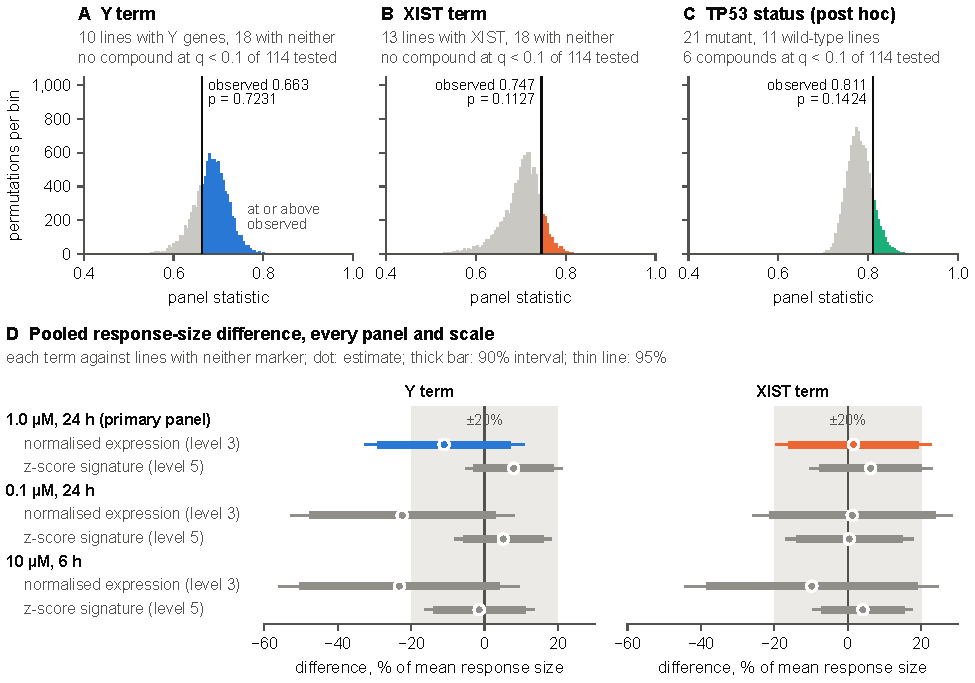
\includegraphics[width=1\linewidth,height=\textheight,keepaspectratio,alt={Figure 4. Part B in the primary panel (1.0 µM, 24 h). A and B, the panel-level statistic, the mean over the 114 tested compounds of the per-compound statistic Tc, for the Y term (A) and the XIST term (B), against its null from 10,000 permutations within lineage; the line marks the observed value (p = 0.7231 and p = 0.1127; rejection needed p \textless{} 0.025). C, a post hoc benchmark with TP53 status as the exposure (p = 0.1424). D, the pooled response-size difference, in percent of the mean response size, for each panel and scale (level 3, each well minus its plate's vehicle wells; level 5, consensus z-scores), with 90\% (thick) and 95\% (thin) intervals and the ±20\% margin (band). Only the primary panel on level 3 carries a decision rule. Lines: 10 express Y genes, 13 XIST and 18 neither, in 11 lineages.}]{figures/fig4_partB.pdf}
\caption{\textbf{Figure 4. Part B in the primary panel (1.0 µM, 24 h).}
A and B, the panel-level statistic, the mean over the 114 tested
compounds of the per-compound statistic T\textsubscript{c}, for the Y
term (A) and the XIST term (B), against its null from 10,000
permutations within lineage; the line marks the observed value (p =
0.7231 and p = 0.1127; rejection needed p \textless{} 0.025). C, a post
hoc benchmark with TP53 status as the exposure (p = 0.1424). D, the
pooled response-size difference, in percent of the mean response size,
for each panel and scale (level 3, each well minus its plate's vehicle
wells; level 5, consensus z-scores), with 90\% (thick) and 95\% (thin)
intervals and the ±20\% margin (band). Only the primary panel on level 3
carries a decision rule. Lines: 10 express Y genes, 13 XIST and 18
neither, in 11 lineages.}
\end{figure}

\subsubsection{Sensitivity of the test (post
hoc)}\label{sensitivity-of-the-test-post-hoc}

The pre-specified positive control, AMG-232 by TP53 status, ranked 1 of
114 (p = 0.0008; Methods). After inspecting the main results, we
assessed panel-level calibration and sensitivity. In simulations with
random labels within lineage, rejection was less frequent than the
nominal threshold for both marker terms. The same panel-level test did
not detect TP53 status across the panel (p = 0.1424; Figure 4C),
although 6 compounds reached q \textless{} 0.1 when analysed separately.

An approximate calculation put the pooled difference needed for 80\%
power at 30.9\% for Y and 30.2\% for XIST. Increasing every drug-response
vector in the labelled group by 20\% led the panel test to reject in
59 of 1,000 assignments for Y and 28 for XIST. The 95\% interval for the
vehicle-referenced pooled difference excluded zero in 301 and 396
assignments, respectively (Figure S3, Note S17). Only
344 of the 4,519 line-by-compound responses used a signature built from
more than one well.

\subsubsection{Pooled response size}\label{pooled-response-size}

On level 3, referenced to vehicle wells on the same plate, pooled
differences were −11.0\% for Y (90\% CI −29.1 to 7.1; 95\% CI −32.8 to
10.8) and 1.6\% for XIST (90\% CI −16.1 to 19.3; 95\% CI −19.7 to 22.9).
Both 95\% intervals included zero (Figure 4D). The Y interval extended
beyond the negative margin. The XIST 90\% interval fell within the
margin, but the planned sensitivity calculation gave only a 0.255 chance
of such an interval under no effect, below the required 0.8. Neither
comparison met the criterion for an equivalence claim.

For Y, the pooled estimate changes sign between level 3 and level 5,
which uses consensus z-scores (Table S12). In post hoc checks,
reassigning or excluding the 3 retained lines with less certain calls
did not change the decision. Removing weakly active compounds moved the
Y estimate toward zero (Note S17). The median per-compound interval
half-width exceeded the effect size of interest for both terms.

\subsubsection{XIST and the vehicle
control}\label{xist-and-the-vehicle-control}

In the XIST comparison, the vehicle control gave p = 0.0323. The count
of compounds with p \textless{} 0.05 was 11, just above the decision
threshold of 10. The panel statistic (0.747) was slightly below the 95th
percentile from a separate random-partition reference (0.748). These
diagnostics, together with the panel and per-compound results, do not
establish an association between XIST expression and compound response.

\subsubsection{Donor labels and named
compounds}\label{donor-labels-and-named-compounds}

The panel-level comparison by donor label also did not reject (p =
0.5544; 25 lines (11 vs 14) in 6 lineages). This comparison includes 5
of 11 male-labelled lines with low Y expression.

Of the four named compound hypotheses, the Y comparison for idarubicin
had an estimated response-size difference of 34.9\% (90\% CI 14.9 to
55.0) across 33 lines (Holm-adjusted p = 0.0160). The separate
per-compound shape test gave p = 0.0446 and q = 0.847. The XIST
response-size estimate had the same direction as Y, consistent with a
difference in the reference group shared by the two contrasts. An
earlier pilot had examined idarubicin at a lower dose, and the later
exploratory check did not reproduce the result in the one testable
condition outside the prior analyses (Notes S17, S18 and S19).

\begin{longtable}[]{@{}
  >{\raggedright\arraybackslash}p{(\linewidth - 8\tabcolsep) * \real{0.1800}}
  >{\raggedright\arraybackslash}p{(\linewidth - 8\tabcolsep) * \real{0.2800}}
  >{\raggedright\arraybackslash}p{(\linewidth - 8\tabcolsep) * \real{0.1800}}
  >{\raggedright\arraybackslash}p{(\linewidth - 8\tabcolsep) * \real{0.1800}}
  >{\raggedright\arraybackslash}p{(\linewidth - 8\tabcolsep) * \real{0.1800}}@{}}
\caption{\textbf{Table 3. Part B: hypotheses, decision rules and
outcomes in the primary panel (1.0 µM, 24 h).} The panel-level and
per-compound tests use level-5 responses, and the pooled response-size
difference uses level 3. The donor-label comparison is
descriptive.}\tabularnewline
\toprule\noalign{}
\begin{minipage}[b]{\linewidth}\raggedright
Test
\end{minipage} & \begin{minipage}[b]{\linewidth}\raggedright
Decision rule
\end{minipage} & \begin{minipage}[b]{\linewidth}\raggedright
Y term
\end{minipage} & \begin{minipage}[b]{\linewidth}\raggedright
XIST term
\end{minipage} & \begin{minipage}[b]{\linewidth}\raggedright
Annotated sex
\end{minipage} \\
\midrule\noalign{}
\endfirsthead
\toprule\noalign{}
\begin{minipage}[b]{\linewidth}\raggedright
Test
\end{minipage} & \begin{minipage}[b]{\linewidth}\raggedright
Decision rule
\end{minipage} & \begin{minipage}[b]{\linewidth}\raggedright
Y term
\end{minipage} & \begin{minipage}[b]{\linewidth}\raggedright
XIST term
\end{minipage} & \begin{minipage}[b]{\linewidth}\raggedright
Annotated sex
\end{minipage} \\
\midrule\noalign{}
\endhead
\bottomrule\noalign{}
\endlastfoot
Lines compared, within lineage & each term against the lines that
express neither marker & 10 against 18 (13 XIST lines also in the model)
& 13 against 18 (10 Y lines also in the model) & 25 lines (11 vs 14) in
6 lineages; male against female label \\
Panel-level test & rejected only if p \textless{} 0.025 & p = 0.7231;
not rejected & p = 0.1127; not rejected & p = 0.5544 \\
Per-compound tests & a finding needs q \textless{} 0.1, a rank in the
top 5\%, a discovery count above 10, and direction and half the size
kept with ploidy and with viability & 0 findings; smallest q 0.684 & 0
findings; smallest q 0.376 & 0 findings; smallest q 0.650 \\
Discovery count, compounds at p \textless{} 0.05 & above 10 (part of the
rules above) & 6 & 11; above the threshold & 5 \\
Pooled response-size difference, \% of the mean response size, level 3 &
a difference only if the 95\% CI excludes zero & −11.0 (90\% CI −29.1 to
7.1; 95\% CI −32.8 to 10.8); none declared & 1.6 (90\% CI −16.1 to 19.3;
95\% CI −19.7 to 22.9); none declared & −6.0 (90\% CI −27.3 to 15.3;
95\% CI −31.9 to 19.8) \\
Equivalence claim & needs a design chance of at least 0.8 that the 90\%
CI falls inside ±20\% & 0.090; no claim & 0.255; no claim & 0.030; no
claim \\
Vehicle negative control (DMSO tested as a compound) & if p \textless{}
0.05, a panel-level result is read as a shift in average response, and
only the per-compound rules can support a compound claim & p = 0.8847
(T\textsubscript{c} rank 98) & p = 0.0323 (T\textsubscript{c} rank 1);
the rule applies & p = 0.2543 (T\textsubscript{c} rank 25) \\
\end{longtable}

\subsubsection{Exploratory follow-ups}\label{exploratory-follow-ups}

Two exploratory vehicle-referenced analyses gave conflicting results for
XIST (Note S18; Table S14). Subtracting a line's level-5 vehicle
response can add a shared component to every compound, which complicates
the interpretation.

\section{Discussion}\label{discussion}

\subsection{Measured expression and donor
labels}\label{measured-expression-and-donor-labels}

The Tahoe-100M vehicle cells show that a donor-sex label can be a poor
proxy for the sex-chromosome genes expressed in culture. The same
distinction matters when RNA-seq comes from a different culture of the
same line. For questions about expression, Table S1 provides the
pattern, culture and call confidence. Calls supported by few cells,
patterns that change across data sources and partial Y expression
warrant additional measurements (Note S9). Donor sex remains relevant to
questions about the donor.

\subsection{Interpretation of the drug-response
test}\label{interpretation-of-the-drug-response-test}

The internally specified LINCS2020 analysis detected no
compound-specific association under its decision rules. The post hoc
calibration checks and broad effect intervals show that the study could
miss differences of biological interest. Performance on the AMG-232
positive control established that the pipeline could detect one large
effect. The panel-level test was insensitive to TP53 status across the
full set of compounds.

The Y estimate was sensitive to response scale. The XIST vehicle result
and conflicting exploratory analyses make the isolated threshold
crossing difficult to interpret. Together, these findings leave the
drug-response question open.

\subsection{Earlier findings by sex in cell
lines}\label{earlier-findings-by-sex-in-cell-lines}

Studies that infer each line's sex-chromosome dosage avoid a mismatch
between expressed patterns and donor labels (Shohat, Vol and Shifman
2022; Plaisier et al.~2025, preprint). Comparisons by recorded sex
(Zeltser et al.~2025, preprint) mix different expression patterns and
can pick up lineage differences or traits associated with marker loss.
Adding Y-gene expression to the label can reduce this risk (Saha et
al.~2024). A Y-gene axis of drug response reflects measured expression
in the cultures assayed.

\subsection{Limitations}\label{limitations}

\begin{itemize}
\tightlist
\item
  \textbf{Cultures and assays.} Part B draws its expression calls from
  other cultures, and different stocks can vary (Ben-David et al.~2018).
  Misclassification unrelated to response can attenuate an association
  (Copeland et al.~1977). AMELY typing in another stock establishes the
  status of one Yp locus in that stock. It cannot show whether other Y
  loci are present or expressed (Cáceres et al.~2020). XIST expression
  can arise from an active X in breast cancer cells (Sirchia et
  al.~2009).
\item
  \textbf{Prior data inspection.} The internal Part B plan followed
  exploratory work with the same data and was held in the analysis
  repository without independent registration. The full Tahoe-100M
  analysis includes the pilot cells. These features limit the evidential
  independence of both analyses.
\item
  \textbf{Cell-level measurements.} Ambient RNA was measured, but the
  pseudobulks were not corrected for it (Note S11). The
  marker-negative-cell analyses could not establish distinct
  subpopulations.
\item
  \textbf{Scope.} The analysis concerns cell lines at the doses and
  times in the panels. It cannot assess hormone-mediated effects or
  pathways that act through T cells (Abdel-Hafiz et al.~2023; Chen et
  al.~2025).
\end{itemize}

A follow-up could assess one contrast: lines expressing Y genes or XIST
versus lines expressing neither, motivated by their shared effects on
autosomal expression (San Roman et al.~2024). It would use expression
measurements from the same cultures as drug exposures, wells as the
experimental units (Huang 2026, preprint), and responses referenced to
same-plate vehicle wells. Demonstrating sensitivity before analysis
would help interpret the result.

\section{Methods}\label{methods}

\subsection{Part A: measured states}\label{part-a-measured-states}

\subsubsection{Data and vehicle cells}\label{data-and-vehicle-cells}

Table S2 lists the sources. In Tahoe-100M (Zhang et al.~2026), vehicle
cells have drug ``DMSO\_TF'' and passed the atlas's full quality filter,
which keeps only cells that genotype-based demultiplexing assigned to a
single line (Zhang et al.~2025, preprint, Methods): 2,205,786 cells in
28 wells on 14 plates, with every line in every well (Note S2). All the
lines but hTERT-HPNE, a telomerase-immortalized pancreatic line, come
from cancers (Bairoch 2018). EmeraldBay and sci-Plex vehicle cells were
analysed separately, using the cut-offs and processing choices specified
for each atlas (Notes S3 and S7). Part A used vehicle cells for scores,
cut-offs and ambient background. External states come from two earlier
analyses of bulk RNA-seq with the same rules: for LINCS2020 lines, CCLE
(Ghandi et al.~2019) first, and for lines screened in GDSC2 or PRISM,
Cell Model Passports (van der Meer et al.~2019) first (Note S1).

\subsubsection{Scores, cut-offs and
patterns}\label{scores-cut-offs-and-patterns}

For a set of cells, the CPM of a gene is its summed UMIs per million
summed UMIs, and each value is the log2 of CPM plus one. The Y score is
the mean of that value over the 8 Y genes RPS4Y1, DDX3Y, KDM5D, UTY,
EIF1AY, ZFY, USP9Y and NLGN4Y; the Yp score uses RPS4Y1 and ZFY, and the
Yq score the other six. Tahoe-100M's primary unit is one line on one
plate (700 units), and a line's call comes from its pseudobulk over all
plates. Each cut-off is the density minimum between the two tallest
modes of a Gaussian kernel density of the line-by-plate values; cut-offs
from line-level values are a sensitivity analysis (Note S3). A score at
or above its cut-off is high.

The two calls give each line a label-independent pattern: Y only, XIST
only, both or neither. The label-dependent comparison combines the
pattern with the Cellosaurus label using Table S3. The release table
retains the original category codes. In the text, low Y and low XIST
refer to expression below the stated cut-off; chromosome structure
requires a separate assay. The Yp and Yq calls give the Y-arm pattern,
read only for male-labelled lines.

A call has high confidence if every plate gives it and it holds when
each cut-off moves by 1 log2 unit up or down, medium if at least 80\% of
plates agree, and low otherwise; lines need at least 200 vehicle cells.
Pooled wells carry ambient RNA, doublets and misassigned cells, so each
pipeline first removed marker-rich cells: cells with 3 or more Y UMIs
from lines with a low Y score, and likewise for XIST. The calls made
before removal equal the final calls, but in lines with partial Y
expression many removed cells are the line's own. The ambient background
is the marker rate in the remaining cells of marker-low lines; for Y, of
lines with both arm scores low (Note S11).

\subsubsection{Implementation and cross-source
agreement}\label{implementation-and-cross-source-agreement}

Two implementations of the same written specification produced the same
expression and confidence calls for all 50 Tahoe-100M lines (Note S4).
This checks how the specification was applied. The cross-source
comparisons in Table 2 assess agreement with other cultures and assays.

A pilot of 26,979 Tahoe-100M cells informed the expression rules and had
already revealed label mismatches. Those cells remain in the full
dataset. The external cultures and their thresholds are described in
Notes S1, S3 and S7. The chronology of the pilot and comparisons is
documented in Notes S8 and S19.

\subsubsection{STR Amelogenin
comparison}\label{str-amelogenin-comparison}

We compared Y-expression calls with AMELY status in short tandem repeat
(STR) profiles compiled by Cellosaurus (Robin, Capes-Davis and Bairoch
2020; release 57.0). Amelogenin typing distinguishes AMELX on the X
chromosome from AMELY on the short arm of the Y (Salido et al.~1992;
Sullivan et al.~1993). Agreement meant a high Y score when AMELY was
detected or a low Y score when only AMELX was detected. This post hoc
comparison covered Tahoe-100M, EmeraldBay and external RNA-seq sources,
and it was also used to assess transfer to the LINCS2020 lines (Note
S14).

\subsubsection{Statistics}\label{statistics}

Agreement proportions are summarized with Clopper-Pearson 95\% intervals
and Cohen's kappa where applicable. The exploratory marker-negative-cell
and depth-matching procedures are described in Notes S5, S6 and S12.
Their cell-bootstrap intervals ignore plate structure.

\subsection{Part B: drug response by measured expression
pattern}\label{part-b-drug-response-by-measured-expression-pattern-1}

\subsubsection{Analysis plan}\label{analysis-plan}

The internal Part B plan specified the hypotheses, models, decision
rules and planned sensitivity analyses before the final analysis joined
marker classes to responses. It was not deposited with an independent
registry. Earlier phases had compared recorded donor sex for 45 of the
115 primary-panel compounds. Pilots had also examined measured markers
and responses, including idarubicin and YM-155 at 0.1 µM. Table S11
separates the original plan from diagnostics and analyses added after
the results were inspected.

\subsubsection{Responses, panels and
states}\label{responses-panels-and-states}

Responses are LINCS2020 L1000 profiles of the 978 landmark genes
(Subramanian et al.~2017). The primary ASG panel contains 115 compounds
plus its DMSO vehicle control. The nominal dose label differs from the
dose recorded for most signatures (1.0 µM at 24 h; Note S16). The
panel-level and per-compound tests included 114 compounds. AZD-8055 had
insufficient lines in a marker group. The low-dose ASG panel (0.1 µM)
and the CPC panel (186 compounds, 10 µM, 6 h) are descriptive because
neither passed a planned positive control.

The unit is the line. A line's response to a compound is the mean over
its signatures on level 5, CMap's consensus z-scores, or over its
treated wells on level 3, where each well is its value minus the mean of
the same plate's DMSO wells, gene by gene. Level-5 z-scores are computed
against the population of wells on the same plate, and each LINCS plate
holds one line, so a line's average response to the compounds on its
plate is largely removed (Note S16). The panel-level and per-compound
tests use level 5, so they test how a line's response to one compound
departs from its response to the others. A difference common to all
compounds is addressed only by the pooled response-size difference, on
level 3.

The states are calls from external RNA-seq, CCLE first (Ghandi et
al.~2019), made as in Part A (Note S1). Lines whose call is discordant
or depends on the source (BEN, HCC1588 and MCF7) were excluded in the
primary plan, and the analysis set keeps the lineages in which a term
varies: 41 lines in 11 lineages (Table S9). The direct comparison of
Y-only with XIST-only lines, closest to the original question, could not
be tested: with 9 lines (4 vs 5) in 3 lineages, the planned analysis
could not calibrate its null (Note S16).

\subsubsection{Model and what each coefficient
compares}\label{model-and-what-each-coefficient-compares}

For each compound and landmark gene, ordinary least squares regresses
the line response on lineage fixed effects, a TP53 covariate (the Cell
Model Passports call, else the CCLE call; van der Meer et al.~2019) and
two state indicators, with t statistics from HC3
heteroskedasticity-consistent standard errors (MacKinnon and White 1985;
Long and Ervin 2000). No line expresses both markers, so the lines fall
into three groups and the model has no interaction term. The Y
coefficient compares lines that express Y genes with lines that express
neither marker, and the XIST coefficient compares lines that express
XIST with the same reference group, within lineage and at the same TP53
status; a positive coefficient means a larger value in the marker group.
The 2 lineages without a reference line, large intestine and soft
tissue, inform the coefficients only through the additive model.

A compound's statistic, T\textsubscript{c}, is the mean of the squared t
statistics over the 978 genes, and the panel statistic is the mean of
T\textsubscript{c} over the tested compounds (each with at least 3 lines
per group). P values come from 10,000 Freedman-Lane permutations within
lineage (Freedman and Lane 1983; Winkler et al.~2014), one set per panel
shared by all compounds and terms (Note S16).

\subsubsection{Positive control and
calibration}\label{positive-control-and-calibration}

Before combining the state and response data, the planned checks tested
AMG-232, an MDM2 inhibitor acting through wild-type p53 (Sun et
al.~2014; Canon et al.~2015), by TP53 status. It had to meet p
\textless{} 0.05 and rank in the top 5\% of compounds. Under random
labels within lineage, the mean fraction of compounds with p \textless{}
0.05 had to lie between 0.03 and 0.07. This assessed the per-compound
tests. Panel-level calibration was examined after the main results (Note
S17).

\subsubsection{Estimands and the interval
method}\label{estimands-and-the-interval-method}

A line's response size s for a compound is the projection of its
response onto the mean response of the other panel lines, scaled so that
a line equal to that mean scores one; it uses no label. It measures
response along the panel's consensus direction, so a line that responds
in another direction has a small s. The estimands are the per-gene shape
effect, the coefficient over the residual SD (effect of interest 1 SD);
the per-compound response-size difference, the coefficient for s in
percent of the compound's mean s (50\%); and the pooled response-size
difference, the coefficient for each line's mean s over compounds in
percent of the mean \emph{s} of the lines in the model, on level 3
(margin ±20\%).

The intervals of the response-size differences are model-based: the
estimate plus or minus the t quantile on the residual degrees of freedom
(27 in the primary panel) times the HC3 standard error, with the mean
\emph{s} treated as fixed. In post hoc simulations, the intervals were
conservative across the tested settings (Note S17).

\subsubsection{Decision rules and error
control}\label{decision-rules-and-error-control}

Table S10 lists each family of tests, its members, its procedure and its
level. The panel-level test uses Bonferroni over the two terms, so each
is rejected only at p \textless{} 0.025. The per-compound tests use
Benjamini-Hochberg within the panel and term (Benjamini and Hochberg
1995). A compound is a finding only if q \textless{} 0.1, its
T\textsubscript{c} ranks in the top 5\%, the number of compounds at p
\textless{} 0.05 exceeds 10, and the 978-gene coefficient vector keeps
its direction and at least half its size, measured by its projection on
the primary vector, after adding ploidy, and after adding the PRISM
viability AUC (Corsello et al.~2020), as covariates (Note S16).
Compounds without a PRISM 19Q4 match, and the 45 compounds on an older
list that earlier phases compared by annotated sex, cannot become
findings.

The pooled response-size difference is an estimate with an unadjusted
decision rule: a difference is declared only if its 95\% CI excludes
zero, and an equivalence claim needs a label-free chance of at least
0.8, under no effect, that the 90\% CI falls inside ±20\%. If DMSO,
tested as a compound, has p \textless{} 0.05 for a term, a panel-level
result for that term is read as a shift in average response. The
donor-label comparison is descriptive. Secondary readouts (Note S17) and
four compound hypotheses named in the plan (trametinib, panobinostat and
vorinostat: Saha et al.~2024; idarubicin) sit outside these families;
each hypothesis is tested at 0.05, with Holm's adjustment over the four
(Holm 1979). Each pre-specified sensitivity analysis changes one choice
of the primary analysis (Table S13).

\section*{Data and code availability}\label{data-and-code-availability}
\addcontentsline{toc}{section}{Data and code availability}

Table S2 identifies the input datasets. Supplementary Table S1 describes
the line-level records, and Note S15 identifies the data terms.
\href{https://github.com/MateenahJAHAN/Project-59-CMAP-Sex-Differences/tree/main/verification}{Result
tables and validation scripts} and
\href{https://github.com/MateenahJAHAN/Project-59-CMAP-Sex-Differences/tree/main/analysis}{analysis
source} are in the project repository.

\section*{Analysis plans}\label{analysis-plans}
\addcontentsline{toc}{section}{Analysis plans}

The Part A rules followed a pilot that included cells in the full
dataset. An internal plan specified the Part B primary model and
decision rules before the final analysis, after exploratory work on the
same data. No independent registry was used. Notes S8, S16 and S19
describe the analysis sequence and prior inspections.

\section*{AI-use statement}\label{ai-use-statement}
\addcontentsline{toc}{section}{AI-use statement}

Claude Code (Anthropic) drafted the expression-calling rules and
analysis plan, wrote and ran analysis code, and prepared figures and
text. OpenAI Codex reran analyses and revised the manuscript. Project
records describe coordination by a non-author and list planned manual
checks for Parts A and B. They do not record which of those checks were
completed.

\section*{Author contributions}\label{author-contributions}
\addcontentsline{toc}{section}{Author contributions}

Mateenah Jahan carried out the earlier CMap and GTEx analyses and
checked the GTEx sign convention (Note S19). Marouen Ben Guebila advised
on the study design and supervised the fellowship.

\section*{Acknowledgements}\label{acknowledgements}
\addcontentsline{toc}{section}{Acknowledgements}

The work took place through the Fatima Fellowship. We acknowledge the
Broad Institute and DepMap for CCLE expression data, the Wellcome Sanger
Institute for Cell Model Passports, the CALIPHO group at the SIB Swiss
Institute of Bioinformatics for Cellosaurus, and Tahoe Therapeutics for
EmeraldBay. Note S15 gives the dataset attributions, licence terms and
transformations.

\section*{Ethics approval and consent to
participate}\label{ethics-approval-and-consent-to-participate}
\addcontentsline{toc}{section}{Ethics approval and consent to
participate}

Not applicable. The study uses public data from established cell lines.

\section*{Keywords}\label{keywords}
\addcontentsline{toc}{section}{Keywords}

Cell lines; sex-chromosome expression; donor-sex annotation; XIST;
perturbation atlas; L1000; Tahoe-100M.

\section*{Abbreviations}\label{abbreviations}
\addcontentsline{toc}{section}{Abbreviations}

CCLE, Cancer Cell Line Encyclopedia; CI, confidence interval; CMap,
Connectivity Map; CPM, counts per million; DMSO, dimethyl sulfoxide;
GDSC, Genomics of Drug Sensitivity in Cancer; LINCS, Library of
Integrated Network-Based Cellular Signatures; RNA-seq, RNA sequencing;
RPKM, reads per kilobase per million mapped reads; STR, short tandem
repeat; UMI, unique molecular identifier.

\section*{References}\label{references}
\addcontentsline{toc}{section}{References}

\begin{itemize}
\tightlist
\item
  Abdel-Hafiz et al.~2023. Y chromosome loss in cancer drives growth by
  evasion of adaptive immunity. Nature.
  \url{https://doi.org/10.1038/s41586-023-06234-x}
\item
  Adduri et al.~2025. Predicting cellular responses to perturbation
  across diverse contexts with State. bioRxiv, preprint, version 2.
  \url{https://doi.org/10.1101/2025.06.26.661135}; journal version:
  \url{https://doi.org/10.1016/j.cell.2026.07.052}
\item
  Adduri et al.~2026. Virtual Cell Challenge 2026: Benchmarking
  zero-shot generalization across cellular contexts. Cell.
  \url{https://doi.org/10.1016/j.cell.2026.08.004}
\item
  Bairoch 2018. The Cellosaurus, a cell-line knowledge resource. Journal
  of Biomolecular Techniques.
  \url{https://doi.org/10.7171/jbt.18-2902-002}
\item
  Ben-David et al.~2018. Genetic and transcriptional evolution alters
  cancer cell line drug response. Nature.
  \url{https://doi.org/10.1038/s41586-018-0409-3}
\item
  Benjamini and Hochberg 1995. Controlling the False Discovery Rate: A
  Practical and Powerful Approach to Multiple Testing. Journal of the
  Royal Statistical Society Series B: Statistical Methodology.
  \url{https://doi.org/10.1111/j.2517-6161.1995.tb02031.x}
\item
  Boulicault et al.~2025. Three maxims for countering sex essentialism
  in scientific research. Biology of Sex Differences.
  \url{https://doi.org/10.1186/s13293-025-00748-x}
\item
  Canon et al.~2015. The MDM2 Inhibitor AMG 232 Demonstrates Robust
  Antitumor Efficacy and Potentiates the Activity of p53-Inducing
  Cytotoxic Agents. Molecular Cancer Therapeutics.
  \url{https://doi.org/10.1158/1535-7163.mct-14-0710}
\item
  Chaligné et al.~2015. The inactive X chromosome is epigenetically
  unstable and transcriptionally labile in breast cancer. Genome
  Research. \url{https://doi.org/10.1101/gr.185926.114}
\item
  Chen et al.~2025. Concurrent loss of the Y chromosome in cancer and T
  cells impacts outcome. Nature.
  \url{https://doi.org/10.1038/s41586-025-09071-2}
\item
  Copeland et al.~1977. Bias due to misclassification in the estimation
  of relative risk. American Journal of Epidemiology.
  \url{https://doi.org/10.1093/oxfordjournals.aje.a112408}
\item
  Corsello et al.~2020. Discovering the anticancer potential of
  non-oncology drugs by systematic viability profiling. Nature Cancer.
  \url{https://doi.org/10.1038/s43018-019-0018-6}
\item
  Cáceres et al.~2020. Extreme Downregulation of Chromosome Y and Cancer
  Risk in Men. JNCI: Journal of the National Cancer Institute.
  \url{https://doi.org/10.1093/jnci/djz232}
\item
  Flynn, Chang and Altman 2021. Large-scale labeling and assessment of
  sex bias in publicly available expression data. BMC Bioinformatics.
  \url{https://doi.org/10.1186/s12859-021-04070-2}
\item
  Freedman and Lane 1983. A Nonstochastic Interpretation of Reported
  Significance Levels. Journal of Business \& Economic Statistics.
  \url{https://doi.org/10.1080/07350015.1983.10509354}
\item
  Gandhi et al.~2025. Tahoe-x1: Scaling perturbation-trained single-cell
  foundation models to 3 billion parameters. bioRxiv, preprint.
  \url{https://doi.org/10.1101/2025.10.23.683759}
\item
  Gertych et al.~2026. Human Y chromosome pan-organ mapping reveals
  progressive mosaic loss from normal to cancer. JCI Insight.
  \url{https://doi.org/10.1172/jci.insight.201996}
\item
  Ghandi et al.~2019. Next-generation characterization of the Cancer
  Cell Line Encyclopedia. Nature.
  \url{https://doi.org/10.1038/s41586-019-1186-3}
\item
  Glass et al.~2013. Passing Messages between Biological Networks to
  Refine Predicted Interactions. PLoS ONE.
  \url{https://doi.org/10.1371/journal.pone.0064832}
\item
  Heidari et al.~2016. Sex and Gender Equity in Research: rationale for
  the SAGER guidelines and recommended use. Research Integrity and Peer
  Review. \url{https://doi.org/10.1186/s41073-016-0007-6}
\item
  Holm 1979. A Simple Sequentially Rejective Multiple Test Procedure.
  Scandinavian Journal of Statistics, volume 6, pages 65 to 70.
  \url{https://openalex.org/W2121044470}
\item
  Huang 2026. Cell lines that share a well are not independent
  observations in the Tahoe-100M drug screen. arXiv, preprint,
  arXiv:2611.01604v1 {[}q-bio.QM{]}, submitted 1 November 2026.
  \url{https://arxiv.org/abs/2611.01604v1}
\item
  Iorio et al.~2016. A landscape of pharmacogenomic interactions in
  cancer. Cell. \url{https://doi.org/10.1016/j.cell.2016.06.017}
\item
  Long and Ervin 2000. Using Heteroscedasticity Consistent Standard
  Errors in the Linear Regression Model. The American Statistician.
  \url{https://doi.org/10.1080/00031305.2000.10474549}
\item
  Lopes-Ramos et al.~2020. Sex Differences in Gene Expression and
  Regulatory Networks across 29 Human Tissues. Cell Reports.
  \url{https://doi.org/10.1016/j.celrep.2020.107795}
\item
  MacKinnon and White 1985. Some heteroskedasticity-consistent
  covariance matrix estimators with improved finite sample properties.
  Journal of Econometrics.
  \url{https://doi.org/10.1016/0304-4076(85)90158-7}
\item
  Masters et al.~2001. Short tandem repeat profiling provides an
  international reference standard for human cell lines. Proceedings of
  the National Academy of Sciences.
  \url{https://doi.org/10.1073/pnas.121616198}
\item
  Müller-Dott et al.~2023. Expanding the coverage of regulons from
  high-confidence prior knowledge for accurate estimation of
  transcription factor activities. Nucleic Acids Research.
  \url{https://doi.org/10.1093/nar/gkad841}
\item
  Nguyen et al.~2026. Recurrent deletions and regulatory disruption of
  the Y chromosome in cancer. Communications Biology.
  \url{https://doi.org/10.1038/s42003-026-10875-9}
\item
  Plaisier et al.~2025. Reproducible autosomal gene expression changes
  with loss of typical X and Y complement across tumor types. bioRxiv,
  preprint. \url{https://doi.org/10.1101/2025.09.24.678401}
\item
  Qi et al.~2023. Loss of chromosome Y in primary tumors. Cell.
  \url{https://doi.org/10.1016/j.cell.2023.06.006}
\item
  Robin, Capes-Davis and Bairoch 2020. CLASTR: The Cellosaurus STR
  similarity search tool - A precious help for cell line authentication.
  International Journal of Cancer.
  \url{https://doi.org/10.1002/ijc.32639}
\item
  Saha et al.~2024. Gene regulatory networks reveal sex difference in
  lung adenocarcinoma. Biology of Sex Differences.
  \url{https://doi.org/10.1186/s13293-024-00634-y}
\item
  Salido et al.~1992. The human enamel protein gene amelogenin is
  expressed from both the X and the Y chromosomes. American Journal of
  Human Genetics, volume 50, pages 303 to 316.
  \url{https://openalex.org/W1492256206}
\item
  San Roman et al.~2024. The human Y and inactive X chromosomes
  similarly modulate autosomal gene expression. Cell Genomics.
  \url{https://doi.org/10.1016/j.xgen.2023.100462}
\item
  Shah, McCormack and Bradbury 2014. Do you know the sex of your cells?
  American Journal of Physiology-Cell Physiology.
  \url{https://doi.org/10.1152/ajpcell.00281.2013}
\item
  Shohat, Vol and Shifman 2022. Gene essentiality in cancer cell lines
  is modified by the sex chromosomes. Genome Research.
  \url{https://doi.org/10.1101/gr.276488.121}
\item
  Sirchia et al.~2005. Loss of the inactive X chromosome and replication
  of the active X in BRCA1-defective and wild-type breast cancer cells.
  Cancer Research. \url{https://doi.org/10.1158/0008-5472.can-04-3465}
\item
  Sirchia et al.~2009. Misbehaviour of XIST RNA in Breast Cancer Cells.
  PLoS ONE. \url{https://doi.org/10.1371/journal.pone.0005559}
\item
  Sonawane 2017. Gene regulatory networks for 38 human tissues. Zenodo,
  data set. \url{https://doi.org/10.5281/zenodo.838734}
\item
  Sonawane et al.~2017. Understanding Tissue-Specific Gene Regulation.
  Cell Reports. \url{https://doi.org/10.1016/j.celrep.2017.10.001}
\item
  Srivatsan et al.~2020. Massively multiplex chemical transcriptomics at
  single-cell resolution. Science.
  \url{https://doi.org/10.1126/science.aax6234}
\item
  Steinlechner et al.~2002. Rare failures in the amelogenin sex test.
  International Journal of Legal Medicine.
  \url{https://doi.org/10.1007/s00414-001-0264-9}
\item
  Subramanian et al.~2017. A next generation Connectivity Map: L1000
  platform and the first 1,000,000 profiles. Cell.
  \url{https://doi.org/10.1016/j.cell.2017.10.049}
\item
  Sullivan et al.~1993. A rapid and quantitative DNA sex test:
  fluorescence-based PCR analysis of X-Y homologous gene amelogenin.
  BioTechniques, volume 15, pages 636 to 641.
  \url{https://openalex.org/W1577564952}
\item
  Sun et al.~2014. Discovery of AMG 232, a Potent, Selective, and Orally
  Bioavailable MDM2-p53 Inhibitor in Clinical Development. Journal of
  Medicinal Chemistry. \url{https://doi.org/10.1021/jm401753e}
\item
  Thangaraj, Reddy and Singh 2002. Is the amelogenin gene reliable for
  gender identification in forensic casework and prenatal diagnosis?
  International Journal of Legal Medicine.
  \url{https://doi.org/10.1007/s00414-001-0262-y}
\item
  van der Meer et al.~2019. Cell Model Passports: a hub for clinical,
  genetic and functional datasets of preclinical cancer models. Nucleic
  Acids Research. \url{https://doi.org/10.1093/nar/gky872}
\item
  Verma et al.~2026a. PIE: Generalizing perturbation effects across
  unseen perturbations, contexts and datasets. bioRxiv, preprint.
  \url{https://doi.org/10.64898/2026.10.02.756297}
\item
  Verma et al.~2026b. PIE\_sources. Hugging Face, data set, revision
  ae4ce64. \url{https://doi.org/10.57967/hf/11208}
\item
  Winkler et al.~2014. Permutation inference for the general linear
  model. NeuroImage.
  \url{https://doi.org/10.1016/j.neuroimage.2014.01.060}
\item
  Zeltser et al.~2025. Sex differences in cancer functional genomics:
  gene dependency and drug sensitivity. bioRxiv, preprint.
  \url{https://doi.org/10.1101/2025.02.05.636540}
\item
  Zhang et al.~2025. Tahoe-100M: A giga-scale single-cell perturbation
  atlas for context-dependent gene function and cellular modeling.
  bioRxiv, preprint, version 1.
  \url{https://doi.org/10.1101/2025.02.20.639398}
\item
  Zhang et al.~2026. Tahoe-100M: Mapping drug-induced molecular
  phenotypes at single-cell resolution. Cell.
  \url{https://doi.org/10.1016/j.cell.2026.08.035}
\end{itemize}

\end{document}
